\documentclass[dvipsnames]{article}
\usepackage{fullpage}
\usepackage[utf8]{inputenc}
\usepackage[T1]{fontenc}
%\usepackage[french]{babel}
\usepackage{tikz}
\usepackage{xcolor}

\title{\vspace{-2cm}Modélisation}
\author{Aurèle Barrière \& Thomas Mari \& Bastien Thomas}
\date{}

\begin{document}

\maketitle

Cette activité est distribuée sous licence CC-BY-SA.

\section{Introduction}
Le but de cet exercice est de faire comprendre qu'il y a plusieurs manières de représenter les mêmes données.
Et que certaines sont plus adaptées à résoudre certains problèmes.
Ici, on donne une description d'un château sous forme de texte, et on veut que les élèves se disent d'eux-mêmes qu'un dessin (graphe) serait plus approprié.
Nous présentons deux versions de l'exercice, pour différents niveaux d'aisance de lecture.
Certaines informations sont superflues. Le but de changer de représentation est aussi de s'initier à filtrer les informations importantes.
Quelques problèmes de graphes sont introduits.
À la fin du document, des graphes sans arêtes peuvent être distribués pour aider à la résolution.

\paragraph{Exercice Introductif}
Si l'intervenant le juge nécessaire, la dernière page comporte un exercice introductif à présenter avant l'exercice principal.
Il s'agit d'une version encore simplifiée (seulement 5 salles) qui permet à l'élève d'appréhender l'exercice.

\section{Questions}
Un mauvais architecte nous a donné une description du château.
La première question à poser:\\
\textbf{La reine se trouve dans sa bibliothèque. Elle aimerait aller dans le grenier, comment peut-elle faire?}

Après quelques temps à essayer, les élèves ne vont pas trouver de solution (il n'y en a pas).
Au bout d'un moment, on leur rajoute l'information suivante:\\
\textbf{Dans la première version des plans, l'architecte avait oublié de préciser qu'il existe une porte entre la salle à manger et la cuisine.}

Si les élèves trouvent la solution, les questions suivantes peuvent être posées:
\begin{itemize}
\item Quel est le chemin le plus rapide?
\item La chambre du roi est fermée, comment peut-elle accéder rapidement au grenier?
\item Le peintre du château aimerait repeindre chaque pièce, de telle sorte que deux pièces adjacentes n'aient pas la même couleur. De combien de couleurs a-t-il besoin, au minimum?
\end{itemize}


\newpage
\section{Description Du Château}
\begin{itemize}
\item Une porte relie la salle à manger et la chambre du roi.
\item Il y a une porte reliant la cuisine et la chambre des servants.
\item La chambre de la reine a une porte donnant sur le jardin.
\item Dans la cuisine, il y a un escalier qui mène au grenier.
\item Depuis la chambre des servants, on peut aller à la buanderie.
\item L'entrée de la tour de guet est dans le jardin.
\item Les chambres du roi et de la reine sont reliées par une porte.
\item La cuisine est reliée à la buanderie.
\item Depuis le Hall d'entrée, un couloir mène à la chambre du roi.
\item Une escalier relie les geôles et la chambre des servants.
\item La porte principale relie le hall d'entrée au jardin.
\item Dans la chambre de la reine, il y a un accès vers la bibliothèque.
\item Du hall d'entrée, on peut aller dans la salle à manger.
\item Dans le grenier, une trappe descend vers la cuisine.
\end{itemize}

\newpage
\section{Description difficile}

Le roi étant gourmand, et n'aimant guère marcher longtemps, une porte reliant sa chambre et la salle à manger s'imposait.
Pour préparer le déjeuner le matin, les servants doivent pouvoir se rendre directement à la cuisine. Ainsi, un couloir étroit relie la cuisine et la chambre des servants.
À la demande de la reine, s'extasiant à la vue d'une floraison printanière, sa chambre fût placée à côté du jardin, et une petite porte lui permet d'y accéder aussi souvent qu'elle le souhaite.
Attention, si vous empruntez l'escalier entre la cuisine et le grenier, la troisième marche est abîmée.
Les servants se plaignent souvent des vapeurs émanant de la buanderie et traversant le petit escalier tortueux qui la relie à leur chambre.
La reine n'aime pas que les soldats traversent régulièrement le jardin pour entrer dans la tour de guet. Malheureusement, c'en est le seul accès.
Tous les soirs, la reine ouvre la porte qui sépare sa chambre de celle du roi, et lui souhaite une bonne nuit.
En attendant qu'un plat finisse de cuire, les servants peuvent passer immédiatement de la cuisine à la buanderie pour s'occuper d'autres tâches.
En rentrant d'une partie de chasse, le roi entre dans le jardin, franchit la grande porte pour passer par le magnifique Hall d'entrée, puis par la porte décorée qui le relie à sa chambre.
Les servants osent rarement ouvrir la petite porte de métal qui mène, depuis leur chambre, aux geôles sordides.
La reine aime se réfugier dans la lecture et le silence de sa bibliothèque. À sa demande, la bibliothèque n'est accessible que depuis sa chambre.
Le Hall d'entrée est vraiment impressionnant. Vous êtes accueillis par des statues imposantes des anciens rois, des plantes grimpantes de taille étonnante qui vous cachent presque la porte qui mène à la salle à manger.
Ce n'était peut-être pas une très bonne idée d'installer cette trappe dans le grenier qui donne sur la cuisine. Plus d'un servant est déjà tombé par mégarde.

\newpage
\section{Exercice Introductif}
Dans cette maison, comment aller du hall d'entrée à la cuisine?
La maison comporte un hall d'entrée, un jardin, une salle à manger, une cave et une cuisine.

\begin{itemize}
\item Le hall d'entrée permet d'aller au jardin ou dans la salle à manger.
\item Depuis le jardin, on peut aussi aller dans la salle à manger ou dans la cave.
\item Il y a une porte qui permet de passer de la salle à manger à la cuisine.
\item On peut aller de la cave à la cuisine.
\end{itemize}


\paragraph{Questions Supplémentaires}
\begin{itemize}
\item Est-ce qu'il y a plusieurs chemins pour aller du hall d'entrée à la cuisine?
\item Quel est le plus court?
\end{itemize}

\newpage
\section{Seconde version: le bateau pirate}

Il y a une porte entre le gaillard d'avant et la réserve de rhum.

Depuis le gaillard d'arrière, il y a des portes pour accéder à la timonerie, à la cambuse et à la cabine du capitaine.
Le capitaine n'aimant pas être dérangé, la porte vers sa cabine est fermée à clef. Cette clef se trouve sur le pont, où le capitaine l'a oubliée.

La timonerie se situe entre la cambuse et la cale, et les trois salles sont reliées par des portillons.

Un escalier relie la cabine du capitaine et la réserve de rhum.

Il y a un échelle de corde qui permet de passer de la cale au gaillard d'arrière. Cependant, pour des raisons de sécurité, on ne peut pas la prendre dans l'autre sens.

Sur le pont, on peut trouver le grand mât. En grimpant sur ce mât on accède au poste de vigie.

Une échelle permet de passer de la cambuse au pont.

Quand ils vont dans leur dortoir, les marins doivent penser à fermer la trappe donnant sur la cale pour ne pas entendre les bruit des rats qui la parcourent. Ils doivent aussi penser à fermer la porte donnant sur le gaillard d'avant pour éviter que le vent ne s'y engouffre.


\paragraph{Questions}
\begin{itemize}
\item Le capitaine se trouve sur le gaillard d'arrière, mais aimerait aller dans sa cabine. Il a aoublié sa clef sur le pont. Quel est le chemin le plus court pour aller dans sa cabine?
\item Le lendemain, le capitaine se trouve dans sa cabine mais a encore oublié sa clef sur le pont. Quel est le chemin le plus court pour retourner au gaillard d'arrière?
\item Un moussaillon est chargé de nettoyer tout le bateau. Il doit donc trouver un chemin qui passe par toutes les salles en partant du poste de vigie. Pour ne pas perdre de temps, il aimerait ne passer qu'une seule fois par chaque salle. Comment doit-il faire?
\end{itemize}

\newpage
\begin{figure}
  \centering
  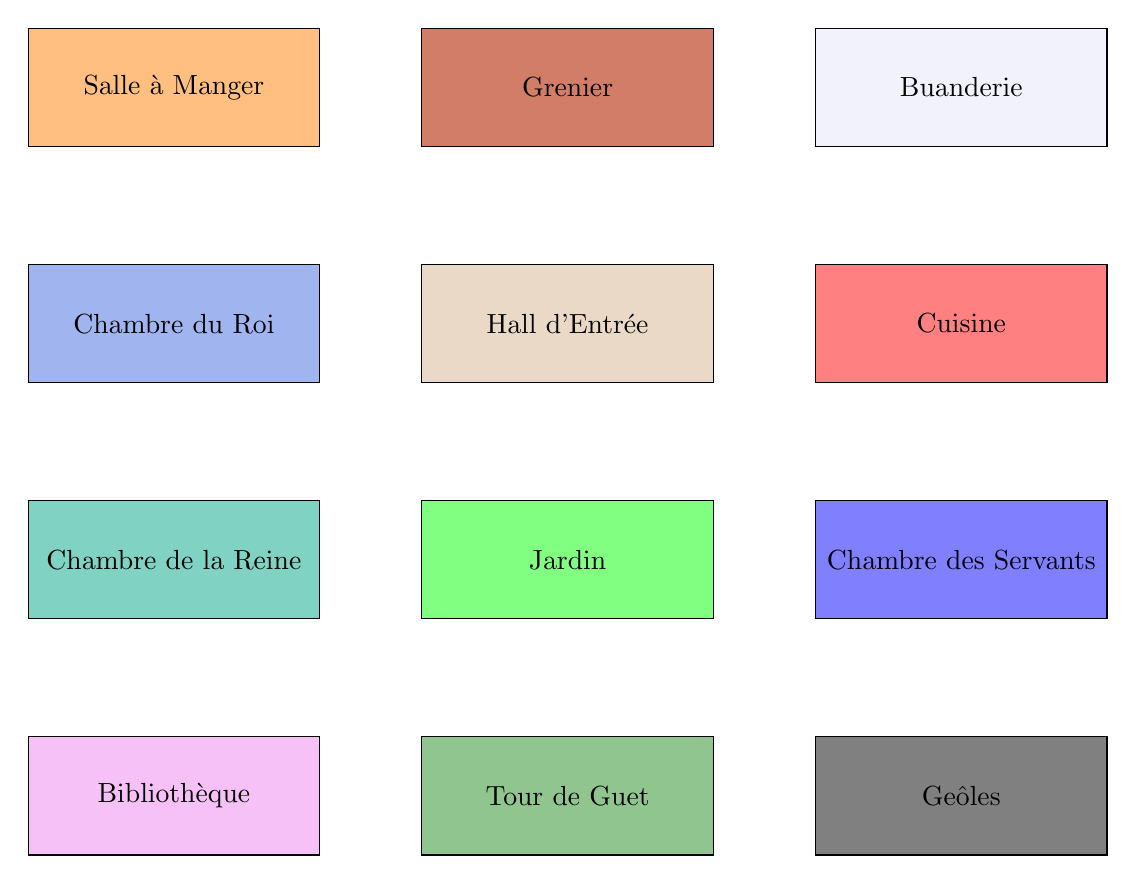
\begin{tikzpicture}
    \node[rectangle, draw=black, minimum height=1.5cm, minimum width = 3.7cm, fill=Violet!50] at (0, 0) {Bibliothèque};
    \node[rectangle, draw=black, minimum height=1.5cm, minimum width = 3.7cm, fill=ForestGreen!50] at (5, 0) {Tour de Guet};
    \node[rectangle, draw=black, minimum height=1.5cm, minimum width = 3.7cm, fill=black!50] at (10, 0) {Geôles};
    %
    \node[rectangle, draw=black, minimum height=1.5cm, minimum width = 3.7cm, fill=Emerald!50] at (0, 3) {Chambre de la Reine};
    \node[rectangle, draw=black, minimum height=1.5cm, minimum width = 3.7cm, fill=green!50] at (5, 3) {Jardin};
    \node[rectangle, draw=black, minimum height=1.5cm, minimum width = 3.7cm, fill=blue!50] at (10, 3) {Chambre des Servants};
  %
    \node[rectangle, draw=black, minimum height=1.5cm, minimum width = 3.7cm, fill=RoyalBlue!50] at (0, 6) {Chambre du Roi};
    \node[rectangle, draw=black, minimum height=1.5cm, minimum width = 3.7cm, fill=Tan!50] at (5, 6) {Hall d'Entrée};
    \node[rectangle, draw=black, minimum height=1.5cm, minimum width = 3.7cm, fill=red!50] at (10, 6) {Cuisine};
    %
    \node[rectangle, draw=black, minimum height=1.5cm, minimum width = 3.7cm, fill=orange!50] at (0, 9) {Salle à Manger};
    \node[rectangle, draw=black, minimum height=1.5cm, minimum width = 3.7cm, fill=Mahogany!50] at (5, 9) {Grenier};
    \node[rectangle, draw=black, minimum height=1.5cm, minimum width = 3.7cm, fill=Lavender!50] at (10, 9) {Buanderie};
  \end{tikzpicture}
\end{figure}

\newpage
\begin{figure}
	\centering
	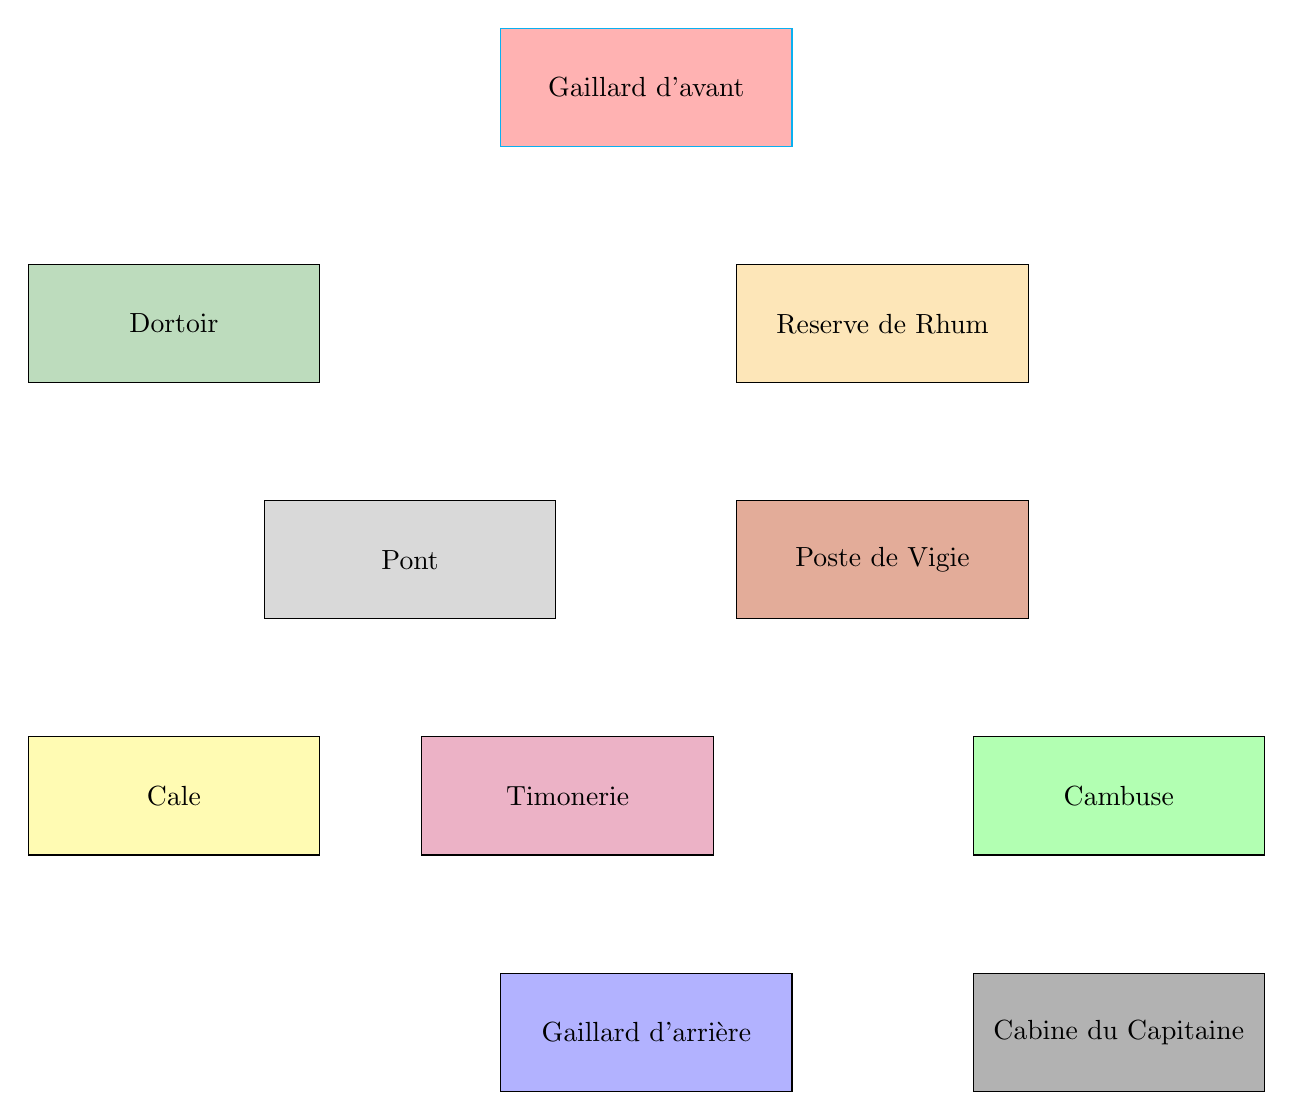
\begin{tikzpicture}
	\node[rectangle, draw=ProcessBlue, minimum height=1.5cm, minimum width = 3.7cm, fill=red!30] at (0, 12) {Gaillard d'avant};
	\node[rectangle, draw=black, minimum height=1.5cm, minimum width = 3.7cm, fill=Dandelion!30] at (3, 9) {Reserve de Rhum};
	\node[rectangle, draw=black, minimum height=1.5cm, minimum width = 3.7cm, fill=blue!30] at (0, 0) {Gaillard d'arrière};
	\node[rectangle, draw=black, minimum height=1.5cm, minimum width = 3.7cm, fill=purple!30] at (-1, 3) {Timonerie};
	\node[rectangle, draw=black, minimum height=1.5cm, minimum width = 3.7cm, fill=Gray!30] at (-3, 6) {Pont};
	\node[rectangle, draw=black, minimum height=1.5cm, minimum width = 3.7cm, fill=green!30] at (6, 3) {Cambuse};
	\node[rectangle, draw=black, minimum height=1.5cm, minimum width = 3.7cm, fill=yellow!30] at (-6, 3) {Cale};
	\node[rectangle, draw=black, minimum height=1.5cm, minimum width = 3.7cm, fill=black!30] at (6, 0) {Cabine du Capitaine};
	\node[rectangle, draw=black, minimum height=1.5cm, minimum width = 3.7cm, fill=Mahogany!30] at (3, 6) {Poste de Vigie};
	\node[rectangle, draw=black, minimum height=1.5cm, minimum width = 3.7cm, fill=ForestGreen!30] at (-6, 9) {Dortoir};
	
	
	\end{tikzpicture}
\end{figure}


\end{document}
